\chapter{Spatio-Temporal Fractal Model for a CPS Approach to Physiological Systems}
\label{cha:ch3}
Advances in the physical sciences and engineering enable the development of cyber-physical systems (CPS) to understand, interface / interact and engineer physical (biological) world (systems). The CPS paradigm refers to a broad class of smart systems with deeply embedded cyber capabilities for sensing, monitoring, and communicating the accumulated large amounts of data about the physical world to computational nodes for real-time analysis, interpretation and determination of closed-loop control strategies \cite{Abdelzaher}\cite{Baheti}\cite{Bogdan}. Although the synergetic coupling of physical and cyber processes has a tremendous impact on a broad application domain (e.g., environmental, healthcare, avionics, smart transportation / buildings / cities), it also raises a few grand challenges: What is the appropriate \textit{modeling framework} that captures the CPS characteristics and facilitates the analysis, design and optimization of CPS? What \textit{compact yet accurate modeling} techniques that account for spatio-temporal complexity and fractal properties should be developed to enable the design of large-scale autonomous (or semi-autonomous) CPS? What are the data mining strategies that meet the real-time CPS requirements? How can the cognitive control of human brain be understood and be enabled within the CPS architectures?

To address these challenges, we turn our attention to biological systems and get inspiration from understanding the dynamics and functionality of human brain to enable a more efficient and safer human-to-cyber-to-physical interaction. From a healthcare perspective, understanding and mining brain activity can be beneficial for developing CPS-based therapies (e.g., brain-machine-body interfaces (BMBI)) for brain disorders. As stated in \cite{He}, we use a rich neurotechnology to measure the brain activity, but lack mathematical models, algorithms and computational tools for understanding neural-muscle data, deciphering disease indicators, explaining brain disorders, identifying clinical therapies and enabling complex human-to-cyber interactions. From control perspective, understanding and modeling the human brain cognition could help us define the principles of autonomous systems design. For manufacturing and smart things, thought-controlled robots that can interact with our collective cognitive efforts could contribute to not only higher yield/performance, but also safer environments. Thought-control systems could prove essential for cleanup operations in dangerous environments (e.g., nuclear reactors) or for maintaining high ecological standards.\\
\begin{figure}%[htb!]
\centering
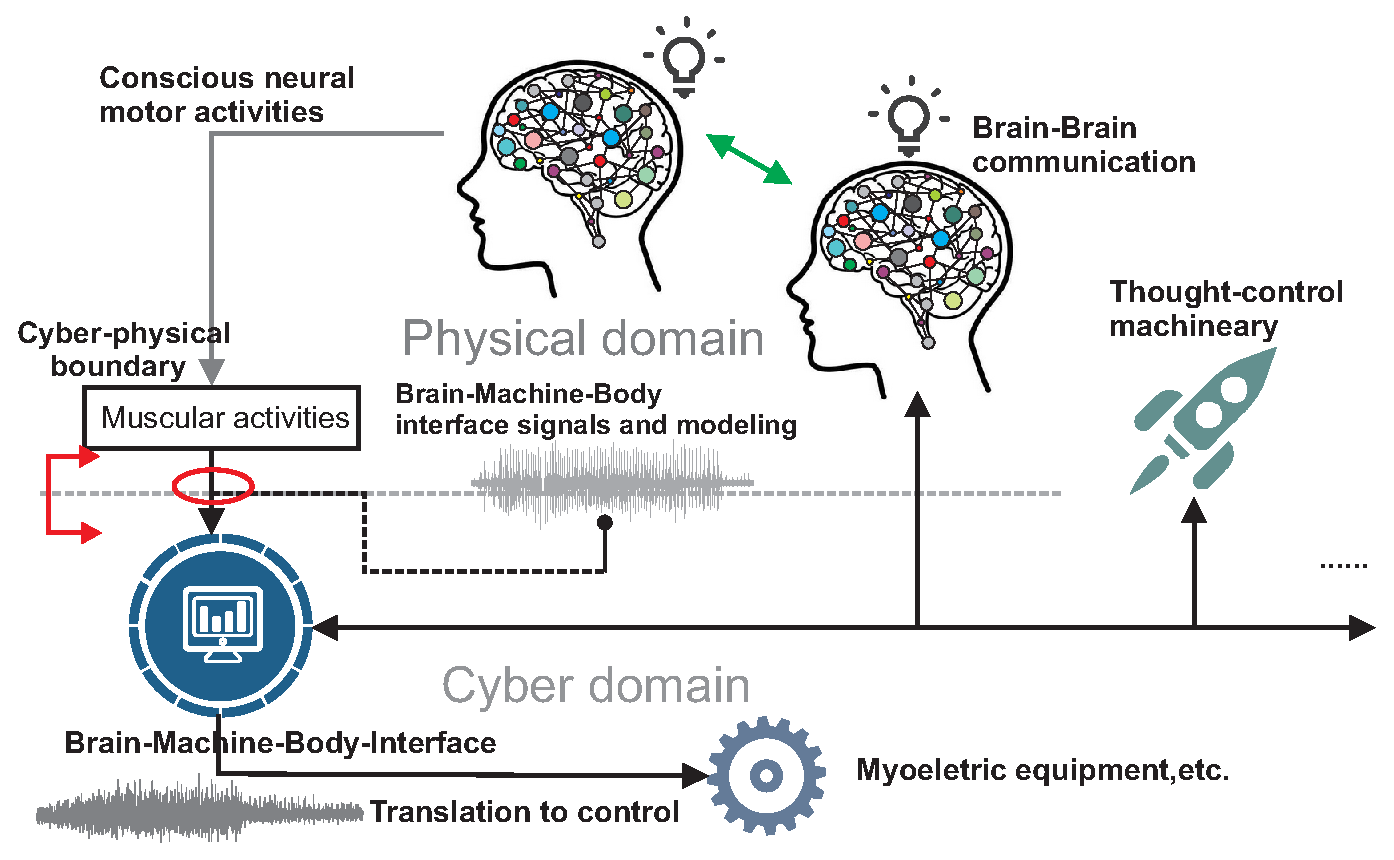
\includegraphics[width=0.94\columnwidth]{brain-brain-interface.eps}
\vspace{-3mm}
\caption{\textbf{Cyber-physcial system for Brain-Machine-Body interfaces}}\label{fig:BMBI}
\vspace{-7mm}
\end{figure}
\indent Traditional approaches for developing decoding algorithms of brain dynamics (converting spiking neural activity from motor cortex into muscle activity and kinematics of a prosthetic arm) have mainly focussed on determining a mapping function from some observations of neural and muscle activity (training data) by minimizing a specific error metric on testing data. Despite some successes, these approaches have neglected some important features of brain-muscle dynamics: (\textit{i}) A cognitive operation may activate a brain region, but the converse operation of activating that same region does not imply that the cognitive process is actually occurring. This implies that assuming instantaneous activation may offer a simplistic view and that the spatial correlation structure and functional dependency between multiple brain regions must be taken into account. (\textit{ii}) Brain activity is not random. Even though many studies assumed a high degree of randomness in the neural dynamics for the purpose of employing statistical averaging, the actual brain dynamics and its coupled physiological processes proved to posses fractal characteristics. Simply speaking, the neural and muscle activity cannot be modeled as short-range dependent processes, but rather their long-range dependence should be accounted for improving modeling accuracy and prediction capabilities. 
\begin{figure} %[htb!]
\centering
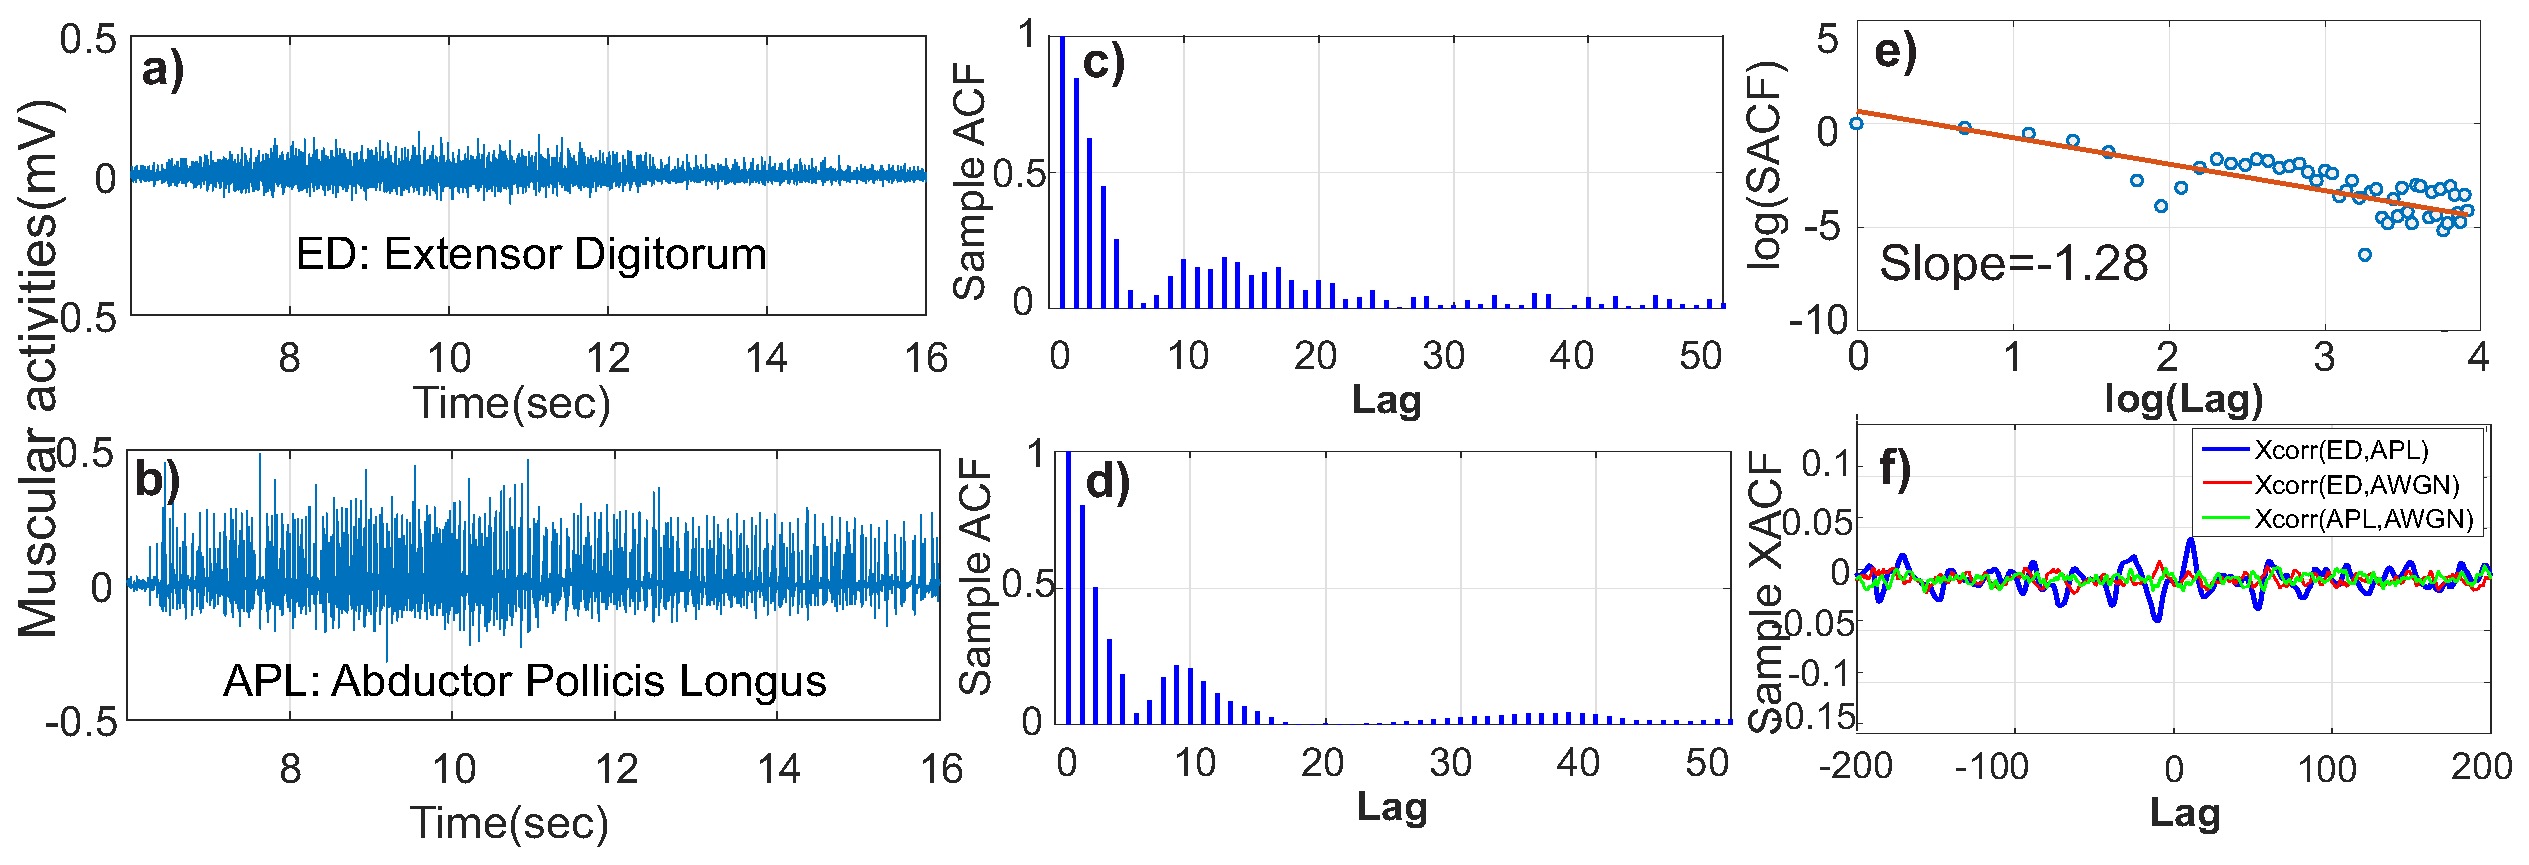
\includegraphics[width=1\columnwidth]{raw_data_thumb_abct_revision.eps}
\vskip -3mm
\caption{\textbf{a-b) The iEMGs from two muscles (ED and APL) are measured when the subject is abducting the thumb for 10 seconds after 6-second relaxing. c-d) The SACF decays hyperbolically rather than exponentially proving a long-range memory. e) The SACF $log-log$ plot of ED iEMG measurements against lags shows a \textit{power-law} behavior. f) The SXACF between the iEMG signals proves the spatial interdependence over time.}}\label{fig:overview}
\end{figure} 
\section{Related Work and Novel Contribution}
Probing brain's activity for the purpose of decoding its cognitive process, explaining its interaction with overall body (e.g., muscles) and controlling the movement of arms originated in the 1960's with the pioneering work of Evarts \cite{Evarts}.  More recently, Donoghue and co-workers designed the BrainGate which allowed a tetraplegic patient with spinal cord injury perform simple movements \cite{Hochberg}.    

Going beyond performing simple tasks requires advanced mathematical and algorithmic approaches for decoding brain-muscle activity. Current approaches for the analysis of electroencephalographic (EEG), electrocortigraphic (ECoG) and electromyographic (EMG) signals can be classified into two classes: linear (e.g., linear estimator \cite{Collinger}\cite{Salinas}, population vector \cite{Velliste}, Wiener filter \cite{Ethier}, Kalman filter \cite{Kim}, recalibrated feedback intention-trained Kalman filter \cite{Fan}) and nonlinear (e.g., artificial neural networks \cite{Sanchez}\cite{Sussillo}, particle filters \cite{Shoham}). 

To enhance the BMBI capabilities and performance, we must address the following challenges: (\textit{i}) Real-time parameter identification of the decoder algorithm. We propose a closed-loop spatio-temporal fractal (STF) model that interacts with BMBI user. This overcomes the suboptimal performance of algorithms that are based on offline cross-correlation validation. (\textit{ii}) Use the neuromuscular spatial dependencies and their fractal dynamics to develop a model of the BMBI at runtime for the purpose of analysis, prediction and control. Many of the current approaches ignore these unique aspects.
%(\textit{i}) Identifying the parameters of the decoder algorithm via offline cross-validation can not only be time consuming, but also lead to poor performance or suboptimal real-time control. Consequently, we advocate for adopting a closed-loop \textit{spatio-temporal fractal} (STF) modeling  approach that continuously interacts with the BMBI user. (\textit{ii}) Many of the current approaches ignore the fractal characteristics and unique aspects of BMBI. In contrast, our STF modeling framework aims to identify the characteristics of the BMBI (spatial dependencies between neural and muscle activity and their fractal dynamics) and develop a model of the BMBI at run-time for the purpose of analysis, prediction and control. %(\textit{iii}) A major problem in CPS based BMBI systems is the state-space explosion (i.e., the number of states required to describe the state of the system tend to increase exponentially). To avoid such situation, we develop an optimization and signal processing algorithmic approach that seeks to determine over predefined windows of time the minimum number of state variables that are required to accurately model and predict the CPS dynamics. 

To illustrate the discrepancies between the mathematical features of biological processes and the current employed memoryless models, we analyze the intramuscular EMG (iEMG) signals from clinical experiments(iEMG Recording study in courtesy of The Alfred Mann Foundation)  where 3 tested healthy subjects are asked to perform forearm movements. The iEMG signals are recorded at different sites of the forearm muscles: (1) extensor digitorum (ED), (2) flexor digitorum profundus (FDP), (3) abductor pollicis longus (APL), (4) flexor pollicis longus (FPL), (5) pronator teres (Pro), and (6) supinator (Sup) (see Figure \ref{fig:exp_setting} and section IV for experimental setup details). Figure \ref{fig:overview} shows 2 measured time series for 2 muscles (ED and APL) when the subject is asked to abduct the thumb at a consistent strength for 10 seconds before relaxing (a-b), the sample autocorrelation function (SACF) of the 2 signals (c-d), the $log$-$log$ plot of SACF of the signal collected from ED (e), and the sample cross-correlation function (SXACF) between the muscle time series (f). The individual analysis of iEMG signals via the SACF method (see Figure \ref{fig:overview}.c-e) shows that the SACF $\gamma(k)$ decreases for higher lags $k$ as a power law rather than as an exponential that corresponds to short-range memory or non-fractal models (including autoregressive (AR) models). This is best shown in Figure \ref{fig:overview}.(e) where the points corresponding to the $log(\gamma(k))$ scatter around a straight line as a function of $log(k)$, following a $log(\gamma(k))=const+\alpha log(k)$ expression. This demonstrates the existence of a correlated neural-muscular regulatory over long temporal horizons. 

To probe the spatial cross-dependency among biological processes, we measure the sample cross-correlation functions (SXACF) (see Figure \ref{fig:overview}.(f)). In contrast to uncorrelated signals (e.g., additive white Gaussian noise with zero SXACF), the SXACF analysis among iEMG signals demonstrates consistent interactive influence and reveals spatial \textit{long-term} dependencies. The amplitudes of the SXACF coefficients are fluctuating over a long temporal horizon which is not expected assuming short memory processes. Such long term memory effect can also be found in other neural and muscular signals and are not discussed here due to limited space. In summary, the analysis in Figure \ref{fig:overview} shows that even the simple movements of the thumb calls for a synergetic model of neural, muscular and cyber components as \textit{interdependent} networks. Alternatively, capturing such long term cross-dependent behavior associated to BMBI calls for the development of \textit{multivariate fractal} mathematical model within CPS. In light of these mathematical observations, we make the following contributions:

\indent \textbf{First}, we propose a \textit{data-driven multivariate fractal} model to capture the long-range memory and spatial cross-dependencies that exist between biological (neural, muscular) and cyber processes. By exploiting the fractal properties of the biological processes, the model can be learned within a CPS infrastructure at run-time from fewer measurements.

\indent \textbf{Second}, we develop an efficient algorithm for identifying the parameters of the proposed mathematical model and provide theoretical bounds concerning the minimum amount of samples that lead to good identification performance.

\indent \textbf{Third}, we investigate the effectiveness and accuracy of the proposed mathematical model, we contrast and highlight the benefits of our model with prior memoryless approaches and validate our model under clinical measurements and known biological facts from medical literature. This mathematical framework enables the understanding of cognitive control and development of advanced control techniques for CPS.   
\section{Spatio-temporal Fractal(STF) Modeling}
%In this section, we start with presenting the biological and physiological foundation of our proposed model by identification of multidimensional correlations that affect the cerebral-muscular synergies of BMBI. To make very concrete discussion, we keep aligning our proposed model with the realistic clinical experiments in capturing the mathematical structures of intramuscular electromyography (iEMG) signal which serves as an important direct information carrier of brain-body signaling system. In the experiments, we evidence the existence of sptio-temporal interplays and fractal properties by analyzing the brain-body interface signals. To best fit to the observed dynamics, we propose a cross-related fractal autoregressive model for characterization of the brain-body synergies. We also develop a joint estimation algorithm for real time analysis to be enforced practically.
\subsection{Premises and Vision for Constructing the STF Model}
The complex interplay between the neural and muscle systems leads to a \textit{closed-loop networked control} architecture that translates bioelectrical signals into motor commands and enables the human body execute highly refined and high degree of freedom movements. Decoding how such translation takes place is essential for BMBI that can further enable brain-to-brain communication and thought-controlled robots. Towards this end, the CPS approach to BMBI shown in Figure \ref{fig:BMBI} needs a mathematical modeling framework for describing brain-body-cyber dynamics and enable human-cyber interactions.

The vision is to build a robust mathematical framework for the CPS approach to BMBI, we represent the interplay between neural, muscular and cyber processes as three highly \textit{dynamic interdependent networks}. From a sensing perspective, the neural activity can be non-invesively sensed via EEG. To quantify the impact of neural commands on muscle activity, we can record the muscle electrical dynamics via EMG signals. Usually two types of EMG signals are recorded: (\textit{i}) The surface EMG (sEMG) signals are used to assess the muscle function from skin level measurements. The sEMGs are influenced by the depth of the subcutaneous tissue at the site of the recording which can be highly variable depending of the weight of a patient, and cannot reliably discriminate between the discharges of adjacent muscles. (\textit{ii}) The iEMG signals avoid the sEMG drawbacks and measure the muscle activity via inserted monopolar or concentric needle electrodes through skin into the muscle tissue. As shown in Figure \ref{fig:overview}, these interdependent networks exhibit: i) A cross-correlated (dependent) spatial patterns when executing different tasks and ii) A complex fractal (long-range memory) property. Consequently, in what follows, we will construct a mathematical model of spatio-temporal fractal interdependent networks.      
%\begin{figure}%[htb!]
%\centering
%\includegraphics[width=0.8\columnwidth]{Rxx_LongRangeDep.jpg}
%\caption{NEED CHANGE ! This figure should be changed and show the long term dependencies of a single channel during thumb %abduction  \label{overflow}}
%\end{figure} 
%\indent Such correlations might invalidate the employment of well-established ICA/PCA based analysis and the autoregressive (AR) models. Neither ICA/PCA based based approaches nor well-established vector AR models could possible capture such spatio-temporal correlations of long term scale as: i) ICA and PCA are instantaneous models, excluding temporal information and quantifying only instantaneous dependencies. However, interactions between muscles are strongly correlated in time. ii) Even though vector AR model consider explicitly the multi-dimensional temporal influence between different physiological processes, the autocorrelation function of its coefficients decays exponentially thus failing to encode the long term memory effect. The failure to understand the comprehensive mathematical signatures of the iEMG signals governing the movement of skeletal muscles may lead to the insufficient or even erroneous control of myoelectric prosthesis resulting in unpleasant user experience or even irreversible consequences. Therefore, for betterment of design human-machine interface (HMI) for movement control of myoelectric prosthesis, it is of primary importance to know the mathematical characteristics of the iEMG signals and establish a model better fitted for estimation, prediction and control.

\subsection{Data-driven Spatio-Temporal Fractal Model}
To build a mathematical model capturing the spatio-temporal fractality among BMBI signals, we denote by $\textbf{X}(t) = [ X_{k_{1}}^{1}(t) ... X_{1}^{n}(t) ... X_{k_{n}}^{n}(t) ]^{T}$,
%\begin{equation}\label{eq:state}
%\mbox{ \textbf{X}(t)} = [ X_{k_{1}}^{1}(t) ... X_{1}^{n}(t) ... X_{k_{n}}^{n}(t) ]^{T}
%\end{equation}
where \textbf{X}($t$) is a $K$-th order STF state vector of $K$ biological and cyber processes representing $n$ different functional entities (e.g. different muscles as in iEMG); the biological and cyber processes interact with each other over time and their cardinality satisfies the following relations: $k_1+k_2+...+k_n=K$; the $X_{k_{l}}^{m}$ is the $k_{l}$-th channel of the $m$-th dimensional BMBI time series. Demonstrated by clinical and experimental investigations, the neural-to-body activities (e.g., body movement) imply a high degree of coordinated dependency among biological entities (e.g., neurons and muscles). To encode such dependencies, we introduce $A(L)^{p}=A_1L+A_2L^2+A_3L^3+$...$+A_pL^p$ as the cross-dependency matrix, where $A_iL^i$ is any $K$x$K$ matrix for which $|A_iL^i|$ has all its root outside the unit circle. Here, $p$ is the autoregressive order that models the \textit{short term} memory effect from events that are $p$-steps back into the past and $L$ is the \textit{backward} operator such that $A_iL^iX_k(t)=A_iX_k(t-i)$. Let $D^{\alpha}(L)$ (with $\alpha=[\alpha_{1},\alpha_{2}$...$\alpha_{K}]^{T}$) be a $K$x$K$ diagonal matrix with entries $(1-L)^{\alpha_{1}}$,$(1-L)^{\alpha_{2}}$,....,$(1-L)^{\alpha_{K}}$, where each $\alpha_{i}\in [-0.5,0.5]$ is the fractal differencing order for $i$-th process. The $D^{\alpha}(L)$ integrates the \textit{long range memory} and can be expressed as a binominal expansion for $k$-th process, $(1-L)^{\alpha_{k}}=\sum_{j=0}^{\infty}\frac{\Gamma(j-\alpha_{k})}{\Gamma(j+1)\Gamma(-\alpha_{k})}L^{j}=\sum_{j=0}^{\infty}\psi(\alpha_{k},j)L^{j}$, where $\psi(\alpha_{k},j)$ is the expansion coefficient that depends only on the fractal order of the process and index $j$. With these definitions, the \textbf{multivariate STF model} reads:
\begin{equation}\label{eq:backward}
D^{\alpha}(L)\textbf{X}(t)=A(L)^p\textbf{X}(t)+\textbf{E}(t)
\end{equation}
\vskip -2mm
\textbf{E}(t)$\sim \textbf{N}(0,\Sigma)$ is a $K$-dimensional multivariate normal distribution with zero-mean and cross-covariance matrix $\Sigma$.
\subsection{STF Model Identification Algorithm}
To jointly estimate matrices $A(L)^p$ and $D^{\alpha}(L)$ (i.e., the fractal differencing operator) of the STF model, we formulate the following optimization problem: 

\textbf{Given} the limited observations of $\{X_{m}(t)\}$ for all $m$ over a time horizon $[t,t+T-1]$ and the following notations: $\textbf{a}_{i}^{m}=[a^{m}_{i,1} a^{m}_{i,2}$...$a^{m}_{i,K}]^{T}$ is the $m$-th row of matrix $A_{i}$, and $Z_{m}(t)=(1-L)^{\alpha_{m}}X_{m}(t)$ represents the fractal differenced time series that is a function of observations $X_m(t)$ weighted by the binominal expansion coefficients.

\textbf{Find} the parameters $[\textbf{a}_{1}^{m} \textbf{a}_{2}^{m}$...$\textbf{a}_{p}^{m}]$ and fractal exponents $\alpha_m$ for all $m$ that minimize the least square error (LSE):
\begin{equation}\label{eq:LSE}
\min\limits_{[\textbf{a}_{1}^{m} \textbf{a}_{2}^{m}...\textbf{a}_{p}^{m}]} \quad\sum_{i=0}^{T-1}(Z_m(t)-\sum_{i=1}^{p}\textbf{a}_{i}^{mT}\textbf{X}(t-i))^2
\end{equation}
\vskip -2mm
%then we propose a multi-variate regression algorithm to solve it.
%and the key steps are : \textbf{1)} We perform Maximally Overlapped Discrete Wavelet Transform for estimation of the fractal differencing order of the model; \textbf{2}) Based on the fractal order estimated, we perform the multivariate regression to give the least square error estimator for the autoregressive correlation matrix.
%\subsubsection{Estimation of long dependency parameter}
%Percival and Walden [ref here] show that a process $X(t)$ with its ACF decaying following a power-law has the variance of its $j_{th}$ scale wavelet coefficients of spectral density function (SDF) $S_{X}(f) \propto |f|^{\alpha}$ as: 
%\begin{equation}
%v^{2}_{y}(\tau_{j}) \propto \tau^{-\alpha-1}_{j}
%\end{equation}
%\begin{equation}
%v^{2}_{y}(\tau_{j})\equiv var\left\lbrace\bar{W}\right\rbrace
%\end{equation}
%\subsubsection{Estimation of the cross correlation matrix}
%Given we have only limited observations of $\textbf{X}(t)$ over time horizon $[t,t+T-1]$. Let $\textbf{a}_{i}^{m}=[a^{m}_{i,1} a^{m}_{i,2}$...$a^{m}_{i,K}]^{T}$ denote the $m$-th row vector of $A_{i}$. Thus if we take the $m$-th BMBI time series $X_{m}(t)$, we have:
%\begin{equation}\label{eq:mrow}
%(1-L)^{\alpha_{m}}X_{m}(t)=\sum_{i=1}^{p}\textbf{a}_{i}^{mT}\textbf{X}(t-i)+e(t)
%\end{equation}
%Let $Z_{m}(t)=(1-L)^{\alpha_{m}}X_{m}(t)$ represent a fractally differenced time series . Therefore, we formulate the estimation problem for cross-dependent coefficient of the $m$-th BMBI signal as an optimization problem:\\
Of note, the fractal differencing order $\alpha_{m}$ of $Z_m(t)$ makes the optimization problem in Eq. (\ref{eq:LSE}) infeasible for applying a linear regression unless we have prior knowledge of $\alpha_m$. Unfortunately, we usually do not have any information about $\alpha_m$ and decoupling the estimation of fractal order from that of $A(L)$ can cause misleading estimation \cite{Sowell}. 

To solve this problem, we rewrite the Eq. (\ref{eq:LSE}) in form of finite binominal expansion of the fractally integrated terms as:
\vspace {-4mm}
%\begin{align*}
%\sum_{j=0}^{\infty}\frac{\Gamma(j-\alpha_{m})}{\Gamma(j+1)\Gamma(-\alpha_{m})}X_{m}(t-j)= & \sum_{k\neq m}^{K}\sum_{i=1}^{p}a_{i,k}^{m}X_{k}(t-i)  \\
% +\sum_{i=1}^{p}a_{i,m}^{m}X_m(t-i)\numberthis \label{eq:bino_expan}
%\end{align*}
\begin{eqnarray}
X_{m}(t)=& \sum_{k\neq m}^{K}\sum_{i=1}^{p}a_{i,k}^{m}X_{k}(t-i)+\sum_{i=p+1}^{inf}\psi(\alpha_{m},j))X_m(t-i)\nonumber \\
&+\sum_{i=1}^{p}(a_{i,m}^{m}-\psi(\alpha_{m},j))X_m(t-i)\label{eq:bino_expan}
\end{eqnarray}
\vskip -2mm
As we know,  $\frac{\Gamma(j-\alpha_{m})}{\Gamma(j+1)}$ is well approximated by $j^{-\alpha_{m}-1}$ when $j$ is large. So we have $\psi(\alpha_{m},j))\sim Cj^{-\alpha_{m}-1}$ where $C$ is a constant. Putting the relation between index $j$ and autoregressive coefficients of $X_m$ in a $log$-$log$ plot leads to a linear function with -$\alpha_{m}$-$1$ slope. This power-law relation not only leads us to our previous argument that our proposed STF model captures the long term dependencies, but also enables us to perform multi-variate regression considering $(K-1)*p+inf$ unknown coefficients to estimate the $A(L)$ and fractal order $\alpha_{m}$ at the same time. Thus we propose an iterative multi-regression algorithm to solve this optimization problem. Letting $\textbf{X}_{m}(t,T)$ be a $T$-dimensional observed output over the interval $[t,t+T-1]$, we have
\vspace {-2mm}
\begin{equation}\label{eq:LSE_2}
\textbf{X}_m(t,T)=\textbf{X}(m,inf) \textbf{A}_{m}+\textbf{e}
\end{equation}
\vskip -2mm
where, $\textbf{X}(m,inf)=\{x_{m}(t-i)\}_{T\times ((K-1)p+inf)}$ is a $T\times (K-1)p+inf$ autoregressive observation matrix. The $i$-th row in \textbf{X}$(m,inf)$ represents all the $p$-order autoregressive terms of (K-1) signals  and $inf$-order autoregressive terms of $X_m$ channel at time $t+i$. $\textbf{A}_{m}$=$[a^{m}_{1,1}a^{m}_{2,1}$...$a^{m}_{p,1}$...$a^{m}_{1,m}$...$a^{m}_{infi,m}$...$a^{m}_{p,K}]^T$ is a vector that contains all the unknown dependency coefficients associated to $m$-th signal. $a^{m}_{i,j}$ is the element at position $ (m,j)$ of $A_i$. Eq.  (\ref{eq:LSE_2}) is a linear system such that we could derive the lower-bound of number of observations we need for estimation of coefficients in our model. To have unique solution, the next condition must be satisfied, $T \geq \ Rank(\textbf{X}(m,inf))=(K-1)*p+inf$.  
%\begin{equation}\label{eq:lower bound}
%T \geq \ Rank(\textbf{X}(m,inf))=(K-1)*p+inf 
%\end{equation}
%\vskip -3mm
Our algorithm could reliably estimate the STF model from few observations as a function of the time series cardinality and model order $p$. This translates in reduced complexity. 
\begin{algorithm}[t]
\caption{LSE Estimator for STF model}
\label{alg:KL}
\begin{algorithmic}[1]
\REQUIRE ~~ Observations $\textbf{X}(t)$; Autoregressive order $p$;
    \ENSURE ~~ Cross dependency matrix set $\{A_{i}|i\in [1,p]\}$; \\
     fractal differencing order $\alpha$   
\FORALL{$X_m(t)$ in $\textbf{X}(t)$}
\STATE Construct $X(m,inf)$
\STATE Construct \textbf{X}$_{m}$(t,T) 
\STATE \textbf{A}$_{m}$=Multiregress(\textbf{X}$_{m}$(t,T),\textbf{X})
\STATE $Y$=log([$a^{m}_{1,m}$...$a^{m}_{infi,m}$])
\STATE [slope intercept]=Fit(log([1:infi]),Y)
\STATE $\alpha_{m}$=-(slope+1)
\STATE Calculate cross dependency matrix
\ENDFOR
\end{algorithmic}
\end{algorithm}
\section{Experiment Setup and Results}
\begin{figure}%[!]
\centering
\includegraphics[width=1\columnwidth]{exp_setting.eps}
\vskip -4mm
\caption{\textbf{The clinical experiments settings. 3 healthy subjects are implanted with fine wire electrodes measuring the iEMG signals when they are asked to do: i) finger extension; ii) finger flexion; iii) pronation iv) supination}}\label{fig:exp_setting}
\end{figure}
 
In this section, we evaluate the effectiveness of our model and study the mathematical characteristics of BMBI under diverse cerebral-muscular interplays through realistic clinical experiments on 3 healthy subjects. Figure \ref{fig:exp_setting} shows 6 targeted muscles (i.e., 2 flexor muscles, 2 extensor muscles, 1 pronator muscle and 1 supinator muscle) of each subject are inserted with fine wire electrodes for measurement purpose. Subjects are asked to relax 6 seconds, then do the following actions: i) finger extension; ii) finger flexion at a consistent strength for 10 seconds or iii) pronate; iv) supinate. The entire process is repeated twice for each movement. The ADInstruments data acquisition system sampled the iEMG at 4 KHz after applying a 2 KHz low pass filter, and a 10 Hz high pass filter to minimize any motion artifacts from electrodes or leads.

In addition, we compare the popular vector autoregressive moving average (VARMA) with our fractal model in terms of sufficiency of capturing the cross-coupled dynamic behavior. We further show that the fractal connectivity could be statistically inferred by analyzing the dependency matrix $A(L)$ in our model. The connectivity extracted by our model can lead to better recognition, prediction and control in CPS architectures.
\subsection{Effectiveness of Spatio-Temporal Fractal Modeling}
\begin{figure}%[!]
\centering
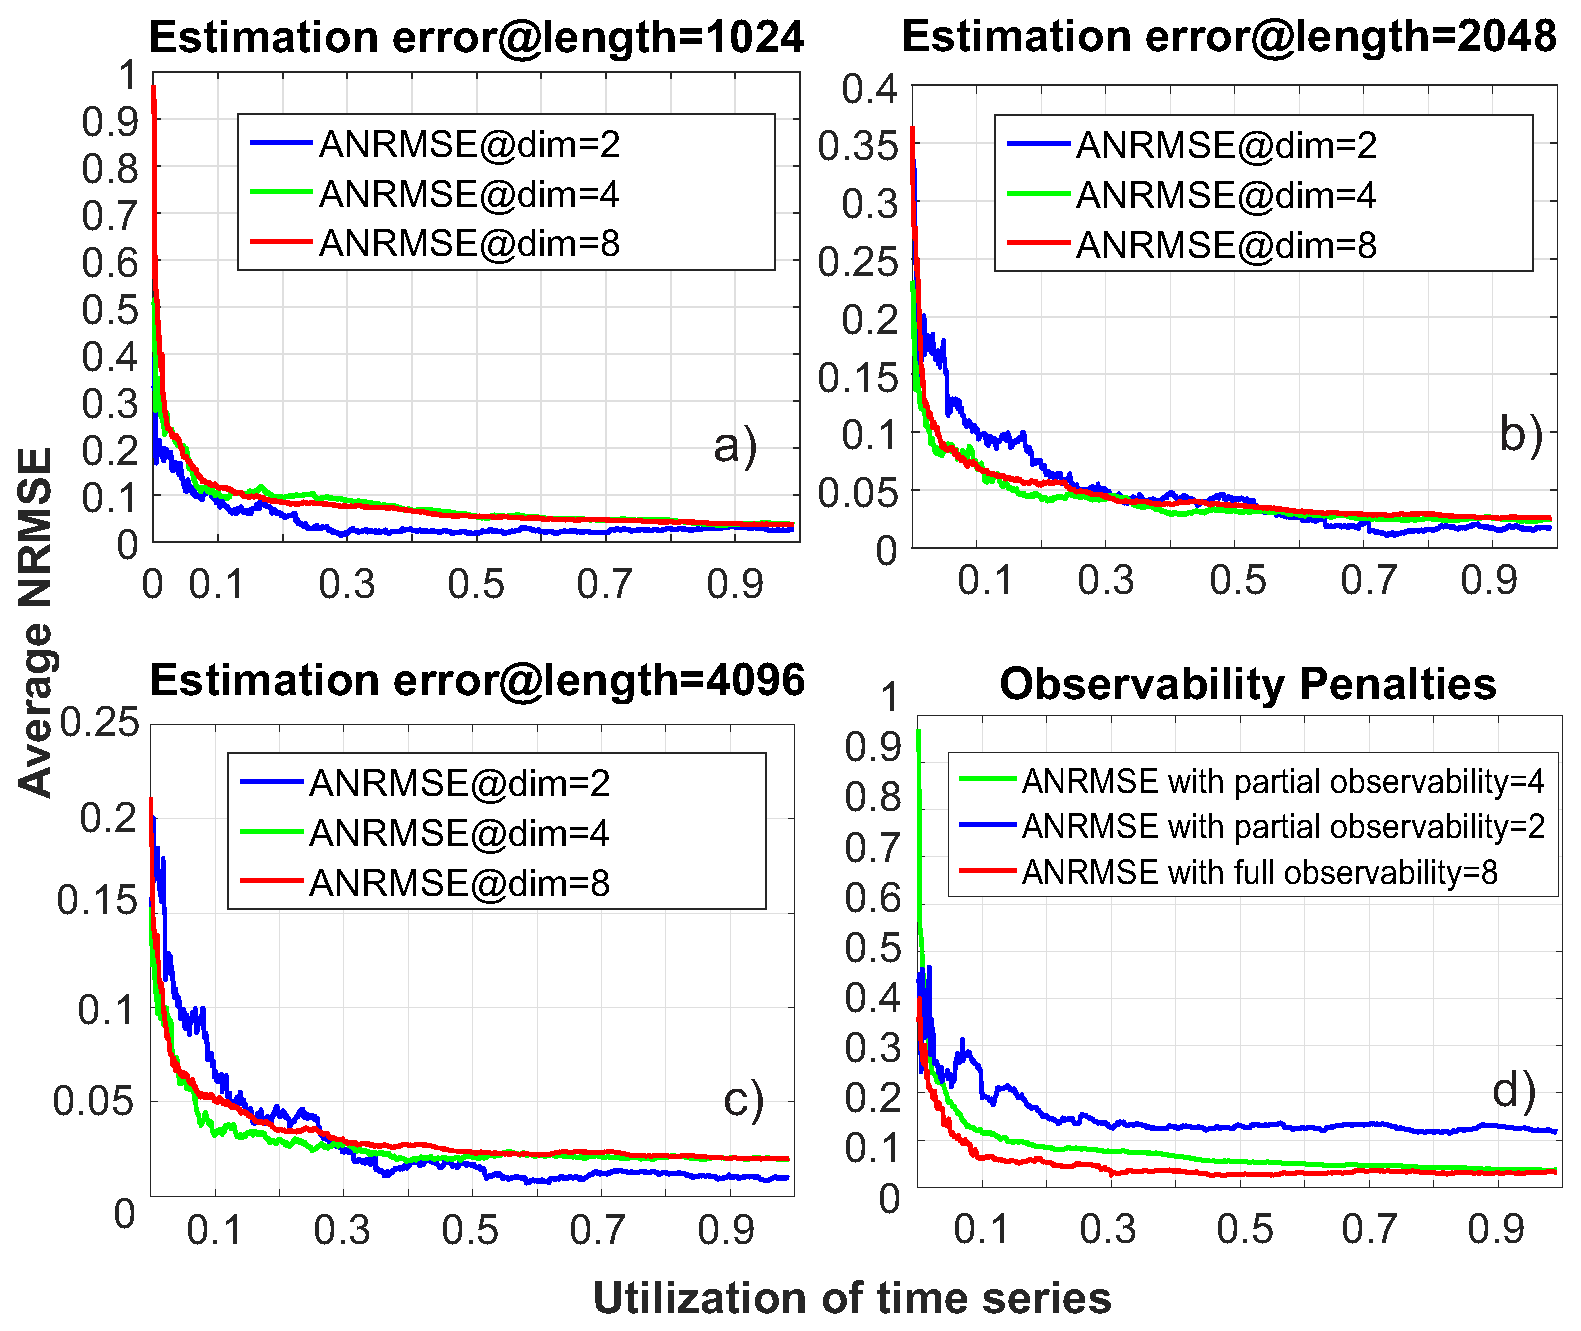
\includegraphics[width=0.95\columnwidth]{effective_algorithm.eps}
\caption{\textbf{The ANRMSE values (a-c) for partial observability of several signal lengths ($1024, 2048, 4096$). d) Partial observability estimating 8-dimensional cross-correlated signals from only $2, 4$ observed channels.} }\label{fig:effective}
\end{figure} 
\begin{figure}%[!]
\centering
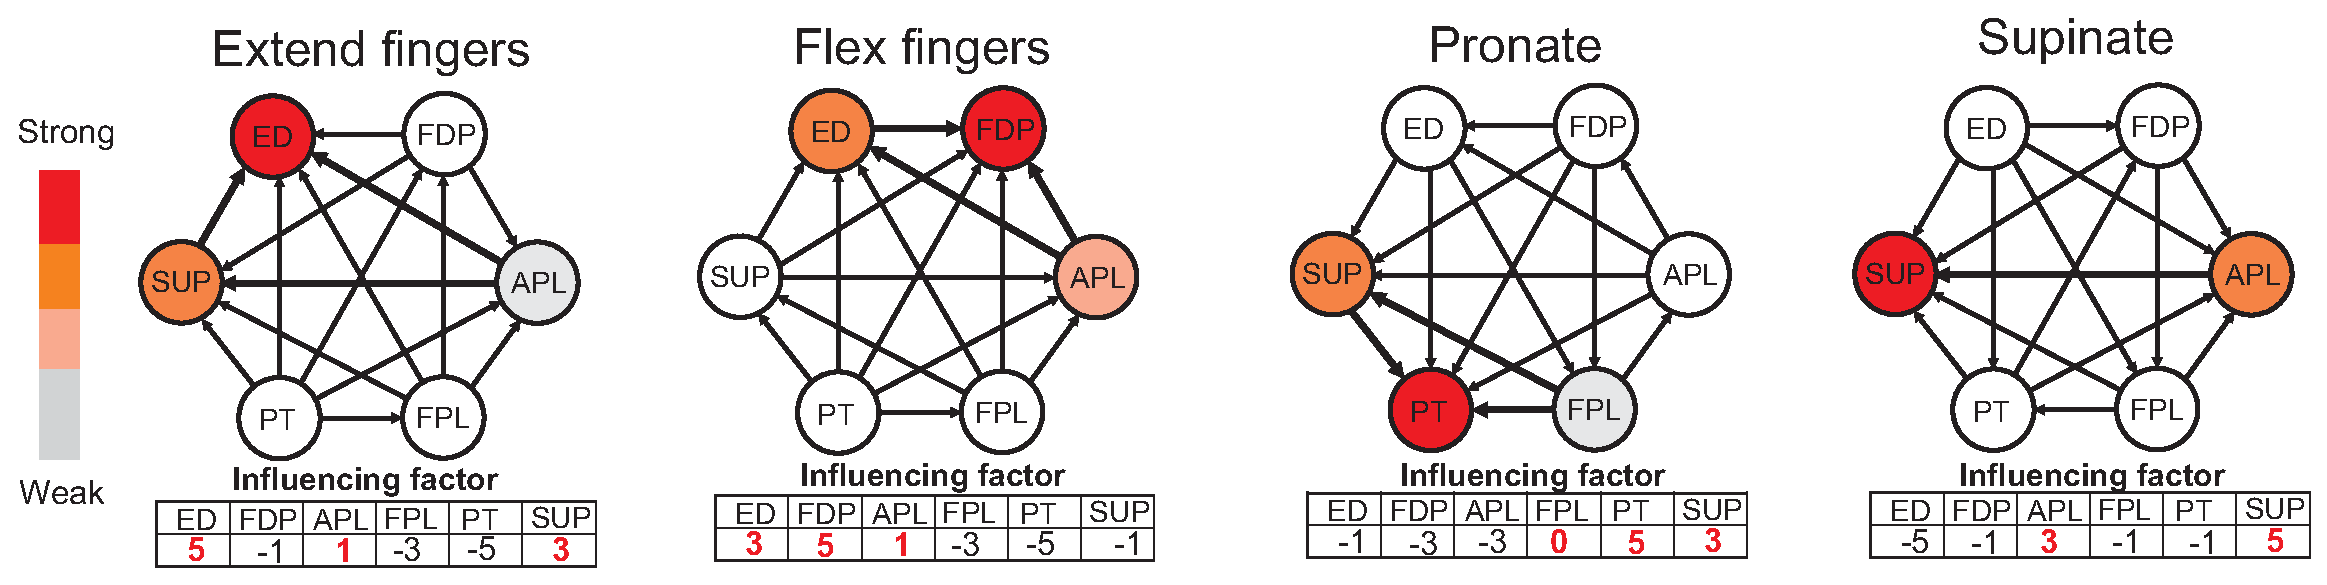
\includegraphics[width=1\columnwidth]{movement.eps}
\caption{\textbf{Fractal connectivity network inferred from 4 different movements. 3 healthy subjects are asked to i) Extend all fingers; ii) Flex all fingers at a consistent strength for 10 seconds or iii) Pronate forearm; iv) Supinate forearm in the experiments. } }\label{fig:movement}
\end{figure}
\begin{figure}%[!]
\centering
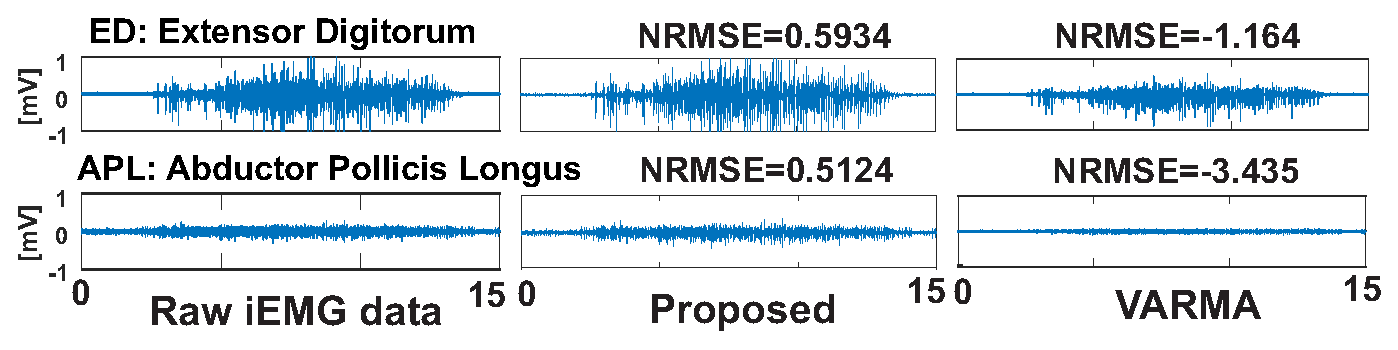
\includegraphics[width=1.0\columnwidth]{comparison_2.eps}
\caption{\textbf{Comparison of first-order model-fitting to 2-channel  (ED and APL) raw iEMG data collected from subject 3 under finger extension} }\label{fig:comparison}
\end{figure}
One major challenge for the design of a CPS approach to BMBI is represented by the need to enable a cyber platform that is able to work with the real-time measurements, identify in real time a compact (few parameters) yet expressive mathematical model and rely on efficient parameter estimation algorithms (determines the mathematical model describing the CPS dynamics from minimum number of samples). This calls for robust and fast algorithms that work with short time series and consistently show good accuracy and fidelity compared to real-time measurements. To justify our proposed framework, we first measure the accuracy of the proposed mathematical identification algorithm in relation to the number of (observed) samples. Then, we show the importance of capturing the spatio-temporal interdependencies of BMBI activities by measuring the deviation in the estimated parameters for two cases: (\textit{i}) The parameters of the model when all the time series are given / observed; (\textit{ii}) The parameters of the model when only a subset of time series are considered.

To investigate the accuracy of the STF modeling framework, we first simulate the proposed model with random choice of $A(L)$ matrix and fractal differencing matrix $D^{\alpha}(L)$ under different signal cardinality (i.e., considering 2, 4 and 8 time series). For each experimental investigation that considers a specific number of time series, we generate 1000 time series of different lengths (i.e., 1024, 2048 and 4096, respectively) and measure the average normalized root mean square error (ANRMSE) between the true and identified parameters as a function of considered number of samples from the initial time series. ANRMSE is calculated as $E[1-\frac{\| \textbf{x}_{ref}-\textbf{x} \|}{\|\textbf{x}_{ref}-E[\textbf{x}_{ref}]\|}]$.

 To obtain the ANRMSE values in Figure \ref{fig:effective}.(a-c), we perform $10^{5}$ experiments for each choice of the number of considered time series, number of considered samples and length of the time series. Simply speaking, we aim to exploit the signals fractality and find the minimum number of samples that would lead to a good model with good accuracy (i.e., the ANRMSE is smaller than a threshold). This would help the CPS to build confidence about the model as the samples are recorded. \\ 
\indent As shown in Figure\ref{fig:effective}.(a-c), the ANRMSE exhibits a phase transition from negligible to noticeable errors as a function of the number of considered samples. For instance, we could use only 30$\%$ of the recordings to learn a good CPS model. In other words, considering only some information about the state-space dynamics represented by the time series (i.e, 10$\%$ or 30$\%$ of the total time series length) the ANRMSE remains almost the same to the case in which more and more samples are included in the identification problem and contributing to higher computational complexity. This can translate into smaller model identification latency and power savings. \\
\indent For many CPS applications, it is important not only to identify a mathematical model with good accuracy from minimum number of samples, but also to be able to retrieve a good model of the system when only a subset of state variables are observed (e.g., reduced order model). In order to study this problem, we consider that from a number of time series  we only know a subset and identify a mathematical model of the form in equation (\ref{eq:backward}). More precisely, we first simulate the proposed model under a cross-dependent model of 8 time series with length of 1024 and generating 1000 trajectories. Then we perform the parameter estimation assuming we only have partial observability (i.e, only consider) to $2$ and $4$ channels from all 8. The ANRMSE values  are reported  in Figure \ref{fig:effective}.(d) as a function of the number of considered samples. As shown in Figure \ref{fig:effective}.(d), when only 4 channels of an 8-dimensional signal representation are observed, the estimation error almost remain the same compared to the case with full observability. It is also noticed that ANRMSE values of the estimated parameters increase noticeably when only two time series out of 8 cross-correlated time series are considered. This implies the failure to model a complex process involving multiple participating entitles (e.g., the cerebral-muscular activities consisting of multiple functional muscles and neurons) and consider sufficient state-variables will lead to model misfitting and biased implication of how these entities are dependent and/or correlated (e.g., the contribution of some muscles in certain movement might be underestimated or overestimated).  
\subsection{Model Validation in Realistic Clinical Experiments}
To investigate the benefits of our model, we compared the goodness-of-fit (GoF) provided by our model and the extensively utilized VARMA model with order $p=1$ when applied to the raw iEMG signals of 6 channels collected from 3 subjects doing different movements. The GoF is quantified in terms of normalized root mean square error (NRMSE) computed for each channel for the two models and averaged over 3 subjects (see Table \ref{tb:fit}). NRMSE is a measure of how well a model fits to the data ranging from $-\infty$ (worst) to $1$ (best). To better illustrate the capability of our fractal modeling approach, Figure  \ref{fig:comparison} summarizes for 2 channels (namely ED and APL when doing finger extension) the comparison between: \textit{i}) First column represents the raw iEMG signals, \textit{ii}) second column denotes the time series generated by our fractal model, and \textit{iii}) third column shows the time series generated by VARMA. As one can notice, VARMA model fits poorly to the raw data with negative NRMSE values. In contrast, our fractal model fits better with NRMSE values over 0.5 for all channels. Table \ref{tb:fit} gives a comprehensive overview of the comparison across all 6 channels from 4 movements. The results consistently show the proposed model gives better fitting over VARMA model. Consequently, our fractal model captures better than VARMA not only the long-range memory of the signals, but also the \textit{cross-dependencies} between signals. Taken together, these results show that modeling fractality can significantly improve not only the GoF of the mathematical model opening the avenue for endowing the CPS with built-in intelligence, but also can lead to a better understanding of fractal properties expressed by biological systems and develop new more efficient control strategies. 
\begin{table}[t]
\center
\caption{Average goodness-of-fit in NRMSE(-inf: worst ; 1 : best)}\label{tb:fit}
\begin{tabular}{|c|c|c|c|c|c|c|c|c|} \hline
\multirow{2}{*}{Channel} & \multicolumn{2}{|c|}{Extend} & \multicolumn{2}{|c|}{Flex} & \multicolumn{2}{|c|}{Pronate} & \multicolumn{2}{|c|}{Supinate} \\
\cline{2-9}
& VA & Frac & VA & Frac & VA & Frac & VA & Frac \\
\hline
ED & -1.2 & 0.52 & -0.86 & 0.47 & -0.15 & 0.30 & -0.65  & 0.46\\
\hline
FDP  & -2.4 & 0.57 & -0.17 & 0.47 & -1.4 & 0.49 & -3.3 & 0.58\\
\hline
APL  & -3.6 & 0.59 & -0.22 & 0.32 & -0.61 & 0.45 & -0.44  & 0.40 \\
\hline
FPL  & -2.5 & 0.55& -1.2 & 0.51 & -9.3 & 0.56 & -2.3  & 0.52\\
\hline
PT  &  -5.9 & 0.59 & -1.8 & 0.54 & -1.0 & 0.50 & -6.2)  & 0.58\\
\hline
SUP  &  -2.7 & 0.57 & -0.13 & 0.25 & -0.33 & 0.36 & -0.37  & 0.55\\
\hline
\end{tabular}
\end{table}
\vskip -2mm
\subsection{Statistical Analysis of Fractal Connectivity}
Fitting the proposed model well to the real neuromuscular processes leads us to several follow-up research directions: i) How can we infer correlations between different participating entities (e.g., different muscles) jointly involved? ii) How can we statistically associate such correlations to specific movements from different subjects in multiple trials to reliably extract patterns? To answer these questions, we exploit the interdependency matrix $A(L)$ and construct the \textit{connectivity network} for pattern recognition. More precisely, we construct the directed graph $G$ from the $A(L)$ coefficients by comparing the off-diagonal coefficients in the symmetric position $(i,j)$ and $(j,i)$ of the matrix with a predefined threshold and drawing directed edge from $j$ to $i$ if muscle $j$ exerts much greater influence on $i$. To deal with variabilities and present reliable patterns, for each connection in $G$, the estimated $A(L)$ coefficients are used to perform a t-test with the null hypothesis that the coefficients come from a distribution with a zero mean (i.e., different muscles are weakly correlated or uncorrelated if no movements are performed). With significance $\alpha=0.05$, the connectivity network is then constructed by including all statistically significant connections, i.e., connections whose $p$-values are smaller than $\alpha$. The resulting connectivity graph for different movements are plotted in Figure \ref{fig:movement}. We quantify the influencing factor $f$ as the difference between the \textit{in}-degree and \textit{out}-degree of a given node. A bigger $f$ is associated with the muscle that is more active in corresponding movement and needs collective assistance from other muscles. The one with biggest $f$ is the dominant muscle in a movement. As one can see from Figure \ref{fig:movement}, our fractal model captures accurately the major dominant muscles involved in all 4 movements and shows consistency with the clinical and anatomical observations \cite{Henry} .
\vskip -7mm
\section{Summary}
In this work, we propose a data-driven fractal mathematical model capable of modeling multi-dimensional cross-dependent BMBI processes with long term dependencies. We justify our model through realistic clinical experiments measuring multi-channel iEMG signals of different natural forearm movements. The comparison between the well-known VARMA and our fractal model shows that our model gives a better fit throughout the experiments. We also statistically infer the fractal connectivity network from the fitted model and show agreement with anatomical observations which lays the foundation for prediction and control of BMBI.